\chapter{The human microbiome and non-alcoholic fatty liver disease}

\section{Introduction}
Non alcoholic fatty liver disease (NAFLD) has been on the rise along with obesity, affecting a fifth to a third of the North American population \cite{preiss2008non}. Most people with NAFLD remain asymptomatic, however, in up to a third of patients NAFLD can progress to non-alcoholic steatohepatitis (NASH), causing inflammation and scarring (fibrosis) in the liver, and decreasing the 5 year survival rate to 67\% \cite{propst1995prognosis}. It is thus important to shed some light on the process by which people progress from NAFLD to NASH to find interventions that prevent NASH.

\subsection{NASH progression risk}
There are several known genetic and chemical factors that increase the risk of progression to NASH in animal models and humans.

\paragraph{Mouse}\mbox{}\\
In mice non alcoholic fatty liver disease is often modelled with a methionine/choline-deficient diet (MCD), which induces steatohepatitis in wildtype mice. Mice with a toll-like receptor 4 knockout had lower lipid and injury accumulation markers when fed a MCD diet \cite{rivera2007toll}.

\paragraph{Rat}\mbox{}\\
In rats liver fibrosis can be induced by drugs. One study found that male rats were more prone to this induced liver fibrosis than female rats. Fibrosis biomarkers were reduced when the male rats were dosed with estradiol, and increased when the male rats were additionally given an estradiol-neutralizing antibody. Female rats who had their ovaries removed similarly lost the protective effect \cite{yasuda1999suppressive}. From this, hormones are also a factor in non-alcoholic fatty liver disease progression.

\paragraph{Human}\mbox{}\\
In humans, the I148M variant of the Patatin-Like Phospholipase Domain Containing 3 gene (PNPLA3) correlates with a 3.2 fold increased risk of progression to NASH from NAFLD when homozygous, compared to to patients without the variant \cite{sookoian2011meta}. The heterozygous gene was found to be associated with fatty liver disease in genome wide association studies, but some additional studies have faileid to replicate the relationship with NASH \cite{sookoian2011meta}.

On the epigenetic level, many genes are differentially methylated in advanced NAFLD compared to mild NAFLD. 11\% of genes are differentially hypomethylated in advanced NAFLD (compared to 3\% hypermethylated), leading to increased expression \cite{murphy2013relationship}. In advanced NASH specifically, some tissue repair genes were hypomethylted while some metabolism pathways such as 1-carbon metabolism were hypermethylated. However, only 7\% of the differentially methylated genes were found to be differentially transcribed \cite{murphy2013relationship}.

On a metabolite level, Raman et al. found differences in the number of volatile organic compounds detected in patients with NAFLD compared to obese patients without NAFLD \cite{raman2013fecal}. Reactive oxygen species have also been implicated in NASH due to their involvement in the mechanism of steatohepatitis-inducing drugs \cite{berson1998steatohepatitis}.

Some groups claim a link between ethanol-producing gut bacteria and NAFLD \cite{zhu2013characterization} \cite{jiang2015dysbiosis}, however the evidence was inconclusive since no multiple test correction was performed.

\subsection{Data}
Applying next generation sequencing techniques to microbiome research is a relatively new field that has yet to set data analysis standards. There are some considerations that should be made when constructing a data analysis strategy.

\paragraph{Data is multivariate}
Generally experiments of this nature typically have low sample sizes due to budget constraints, sample collection difficulties, patient compliance, and other issues.

As a result, the number of taxa or gene functions comparisons made are often a magnitude larger than the sample size. This is known in statistics as having more variables than observations, or having fat data. The higher the ratio of variables to observations are, the less likely standard statistical techniques are to be reliable \cite{osborne2004sample}.

Researchers should include multiple test corrections to ensure that the results they are reporting are true, at the expense of having p-values less than 0.05. Unfortunately many studies have been published in high impact journals without multiple test corrections, including a famous paper linking the gut microbiome to autism published in Cell \cite{hsiao2013microbiota}.

\paragraph{Data is compositional}
In both gene tag sequencing and metagenomic sequencing experiments, the data is in the form of a list of counts per feature, with the features composing an aspect of the microbiome for each sample. This is compositional data. The total number of reads yielded by the sequencing platform is often platform-dependant and not biologically relevant.

This constrained sum causes the abundance of different taxa to appear to be negatively correlated with each other when analyzed by conventional statistics. When one taxa increases in abundance, the counts detected in other taxa decrease in abundance, even if the taxa are not decreasing in abundance biologically.

Compositional data should be analyzed in a compositional way. In Euclidean space, data points can increase or decrease freely. Compositional data is under a sum constraint, and exist in a non-Euclidean space known as the Aitchison simplex \cite{aitchison1982statistical}. Data transformations such as the centered log ratio can be performed to put the data into Euclidean space, so that it can be analyzed with standard statistical methods that depend on Cartesian coordinates and linear relationships.

However, these techniques are not yet mainstream in the field, resulting in a high number of conclusions made that are not reproducible.

\subsection{Literature}
Several papers have already been published in the literature on the topic of NAFLD and the gut microbiome:

\begin{figure}[h]
\begin{center}
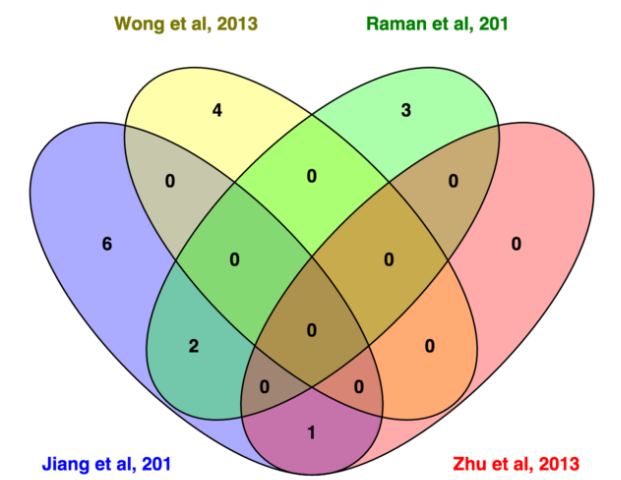
\includegraphics[width=0.7\textwidth]{nafld_papers.png}
\caption{\textbf{Venn diagram of genera found to be differentially abundant by different studies between NASH/NAFLD and healthy controls.} Only 3 out of the 16 genera claimed to be differentially abundant were found in two studies: members of the \textit{Escherichia} genus were found in the Zhu \cite{zhu2013characterization} and Jiang \cite{jiang2015dysbiosis} studies, and members of the \textit{Lactobacillus} and \textit{Oscillibacter} genus were found in the Jiang \cite{jiang2015dysbiosis} and Raman \cite{raman2013fecal} studies.}
\end{center}
\label{nafld_fig1}
\end{figure}

\begin{itemize}
\item Jiang et al, 2015 \cite{jiang2015dysbiosis} compared 53 NAFLD patients with 32 healthy controls

\item Zhu et al, 2013 \cite{zhu2013characterization} compared 16 non-obese controls, 25 obese patients, and 22 NASH patients

\item Raman et al, 2013 \cite{raman2013fecal} compared 30 NAFLD patients with 30 healthy controls

\item Wong et al, 2013 \cite{wong2013molecular} compared 16 NASH patients with 22 healthy controls

\item Boursier et al, 2015 \cite{boursier2016severity} compared 30 patients with F0 or F1 fibrosis to 27 patients with F2 or greater fibrosis, 35 of which had NASH
\end{itemize}

Fig.~\ref{nafld_fig1} shows a Venn diagram illustrating the inconsistency of the literature on the gut microbiome and NAFLD. Of these, only Raman et al \cite{raman2013fecal} reported using a multiple test correction.

Since these five studies do not form a consistent story about the gut microbiome and NAFLD, we conducted own analysis rigorously, such that our results are replicable. Additionally, we generate the first deeply sequenced metagenomic sample set to examine functional capabilities in this disease.

\FloatBarrier

\section{Methods}
In total, 92 samples were collected: 41 from patients with NASH, 18 from patients with SS, and 33 from healthy controls.

[TO DO: include information about sample collection and exclusion criteria]

DNA extraction was performed with the \href{http://omegabiotek.com/store/product/stool-dna-kit/}{E.Z.N.A.® Stool DNA Kit}, and the protocol was followed with the addition of lysozyme with an extra 30 minute incubation at 37 degrees Celcius, between steps 2 and 3.

\subsection{16S rRNA gene tag experiment}

DNA was amplified by PCR according to the Earth Microbiome protocol \cite{caporaso2012ultra}, with the addition of barcodes so that all the samples could be sequenced in the same sequencing run \cite{gloor2010microbiome}. The DNA was sequenced on the Illumina MiSeq platform with paired end 150 nucleotide reads, producing 34955148 reads in total.

Reads were overlapped with Pandaseq \cite{masella2012pandaseq}, clustered into Operational Taxonomic Units using UCLUST \cite{edgar2010search}, and annotated with the SILVA database \cite{quast2013silva}, producing a table of counts per operational taxonomic unit per sample. 16809756 reads (48\%) were succesfully overlapped and annotated with 232 OTUs. Differential abudance was analyzed using ALDEx2 \cite{fernandes2014unifying}.

\subsection{Metagenomic experiment}

A deep metagenomic sequencing experiment was performed using samples from 10 healthy controls and 10 of the patients with NASH. Samples from healthy patients were selected to exclude confounding factors, such as having a different country of birth, which could affect diet. Samples from NASH patients were selected for the strongest NASH phenotype.

The DNA was sequenced on the Illumini HiSeq platform, with single end 100 nucleotide reads. Samples were barcoded and sequenced on the same sequencing run. After sequencing, the reads were quality filtered and demultiplexed to separate the reads for each sample, yielding 1914714572 reads in total.

To annotate the reads, we used a two pronged strategy:

First, we created a reference library using the inferred taxa from the 16S rRNA gene tag experiment. For each genus the OTUs were annotated with, we randomly picked 10 strain genomes from the NCBI bacterial genome database. For genus where there were less than 10 fully sequenced representatives, we selected all genomes available. The library was made with 1134 genomes from 104 bacterial genus. The library was then clustered at 99\% identity for each genus using CD-HIT \cite{li2006cd} to decrease the number of sequences in the library from 3495887 to 2256844. Annotation was performed with the SEED database \cite{overbeek2005subsystems}, and sequenced reads were mapped onto this library. Out of 1914714572 reads total, 585382507 (30.6\%) were annotated by this method, over 5836 unique SEED hierarchy annotations. The code for the \href{https://github.com/ruthgrace/make_functional_mapping_library}{reference library creation} and \href{https://github.com/ruthgrace/mapping_library_annotated_counts}{annotation} is on GitHub.

Second, we assembled the reads per sample de novo using Trinity \cite{haas2013novo}, producing 8847816 sequences, and removed sequences that matched our reference library with 90\% identity as determined by BLAST \cite{altschul1990basic}, leaving 5876423 sequences. [FILL IN THIS] of these assembled sequences were successfully annotated with the SEED database \cite{overbeek2005subsystems}, and sequenced reads were mapped onto this. [FILL IN THIS] additional reads were annotated by this method, over [FILL IN THIS] unique SEED hierarchy annotations. The code for the custom assembly pipeline is on \href{https://github.com/ruthgrace/exploring_nafld_assembly}{GitHub}. The data from both prongs was amalgamated into a single table of counts per annotation per sample.

Differential abudance was analyzed using ALDEx2 \cite{fernandes2014unifying}.

\subsection{MetaPhlAn}

MetaPhlAn (Metagenomic Phylogenetic Analysis) \cite{segata2012metagenomic} is a piece of software that allows one to infer the taxa present based on the metagenomic sequencing experiment. We used this to generate a count table per taxa per sample, and will compare it to our experimental results from the 16S rRNA gene tag sequencing experiment.

\section{Results}

\subsection{16S rRNA gene tag experiment}
The top five genus detected by 16S rRNA gene sequencing (excluding unclassified bacteria) were: \textit{Incertae Sedis}, \textit{Bacteroides}, \textit{Faecalibacterium}, \textit{Blautia}, and \textit{Pseudobutyrivibrio} (Fig.~\ref{nafld_16s_barplot}).

\begin{figure}[h]
\begin{center}
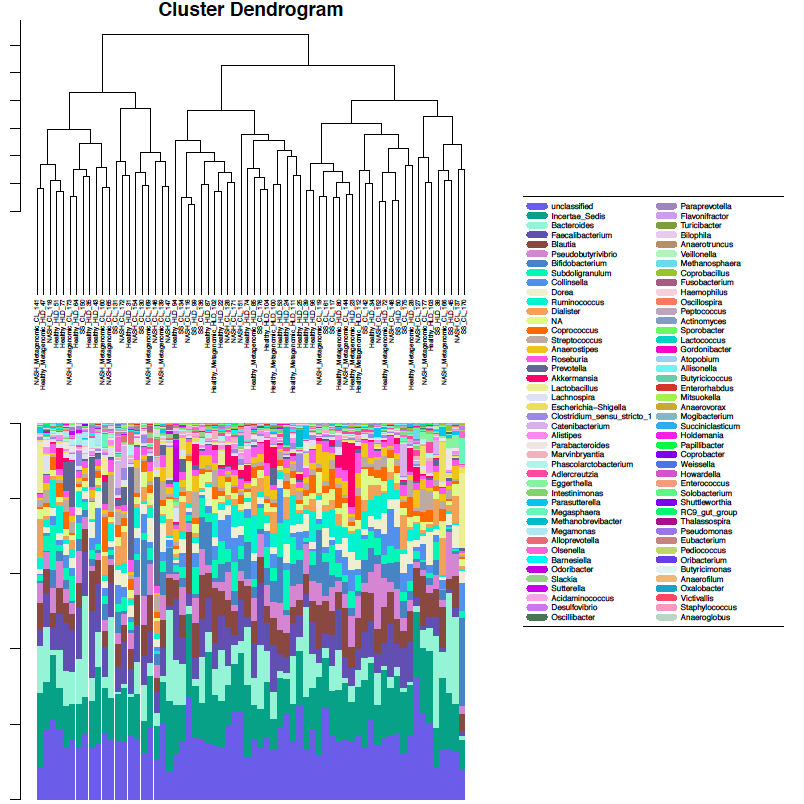
\includegraphics[width=0.95\textwidth]{16s_genus_barplot.png}
\caption{\textbf{16S rRNA gene tag sequencing per sample bar plot.} Each column of this bar plot represents one sample, and each color represents one bacterial genus. Genus are listed in the legend in order of decreasing total abundance across all samples. Samples do not cluster according to their condition (healthy, simple steatosis, or nonalcoholic steatohepatitis).}
\end{center}
\label{nafld_16s_barplot}
\end{figure}

No obvious structure or separation is evident from the principal components analysis in Fig.~\ref{nafld_fig2}. Furthermore the variance explained by each principal component axis is not notably high, indicating a rather uniform data set. Additionally, no OTUs are significantly differentially abundant between groups (Fig.~\ref{nafld_fig3})

\begin{figure}[h]
\begin{center}
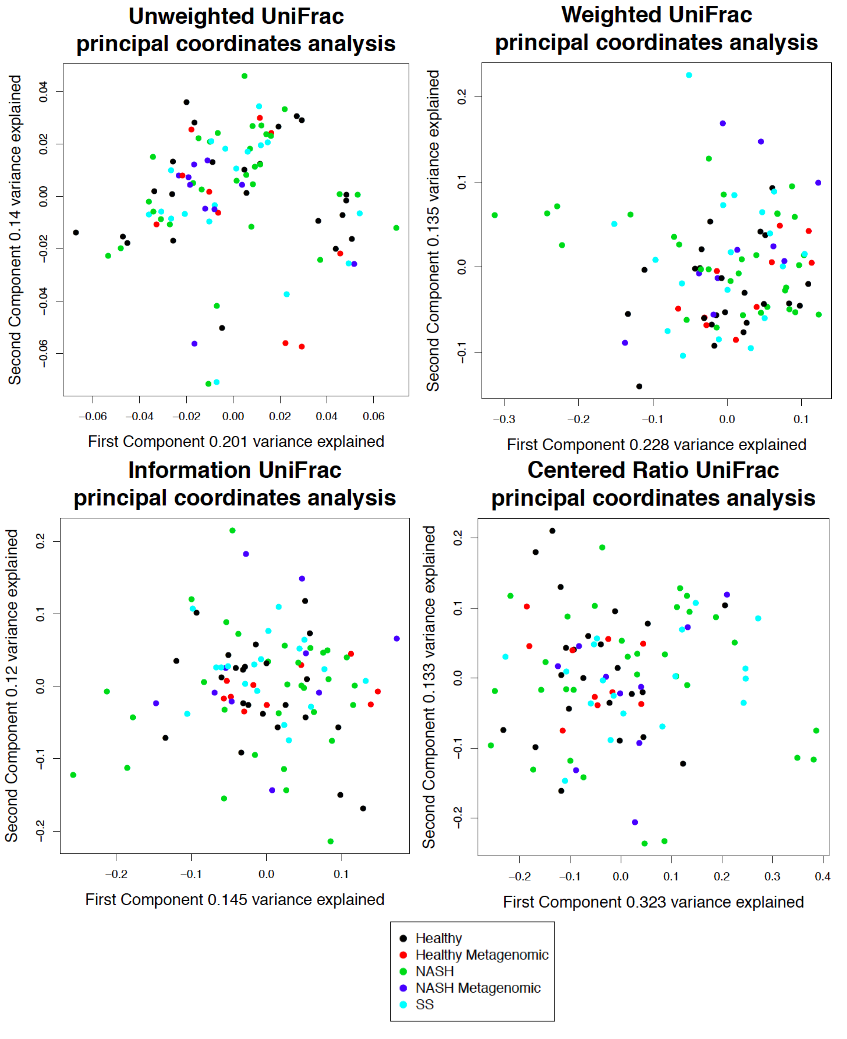
\includegraphics[width=0.95\textwidth]{nafld_16s_pcoa.png}
\caption{\textbf{Principal Components Analysis of 16S rRNA gene tag sequencing data with different UniFrac weightings.} Each point represents one sample, and the distances between the samples have been calculated using different UniFrac metrics, taking into account phylogenetic as well as abundance information. There is no obvious separation between groups by any of the UniFrac weightings. Furthermore the variance explained by each principal component axis is not notably high, indicating a rather uniform data set.}
\end{center}
\label{nafld_fig2}
\end{figure}

\begin{figure}[h]
\begin{center}
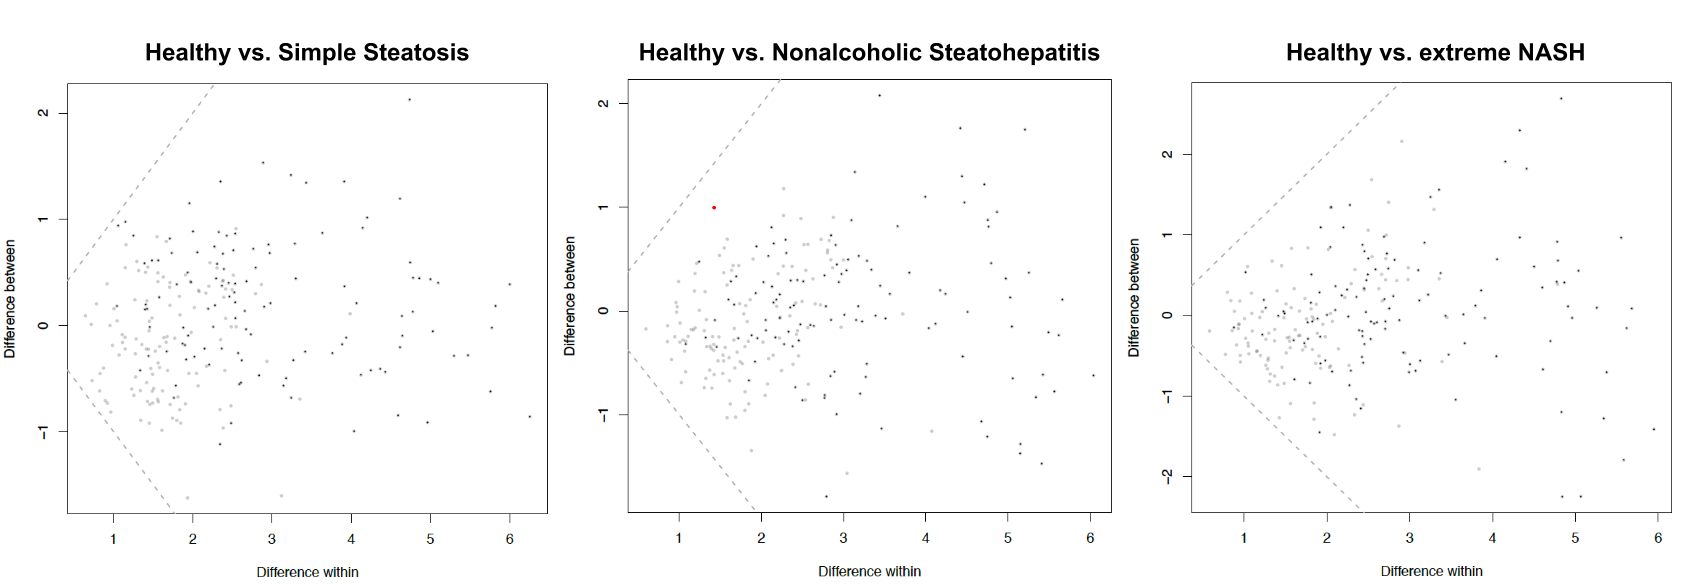
\includegraphics[width=0.95\textwidth]{nafld_16s_aldex.png}
\caption{\textbf{Difference within vs. difference between groups.} Each point represents one OTU, and the differential abundance of that OTU within groups is plotted against the differential abundance between groups. None of the OTUs are more different between groups than within groups. The healthy samples used for these comparisons are the 10 healthy samples used for the metagenomic study. The extreme NASH samples used for these comparisons are the subset of the NASH patients selected for the metegenomic study.}
\end{center}
\label{nafld_fig3}
\end{figure}

When comparing all the healthy samples with all the NASH samples, the genus with the highest effect sizes are \textit{Adlercreutzia}, \textit{Odoribacter}, and \textit{Escherichia-Shigella}. However, when only the select 10 healthy samples and the 10 extreme NASH samples used in the metagenomic study are compared, the genus with the highest effect sizes are \textit{Ruminococcus}, \textit{Adlercreutzia}, and \textit{Alistipes}. This corresponds with the qPCR experiment, where \textit{Bacteriodetes}, \textit{Prevotella}, and \textit{Ruminococcus} were tested, and only \textit{Ruminococcus} was found to be differentially abundant.

\begin{figure}[h]
\begin{center}
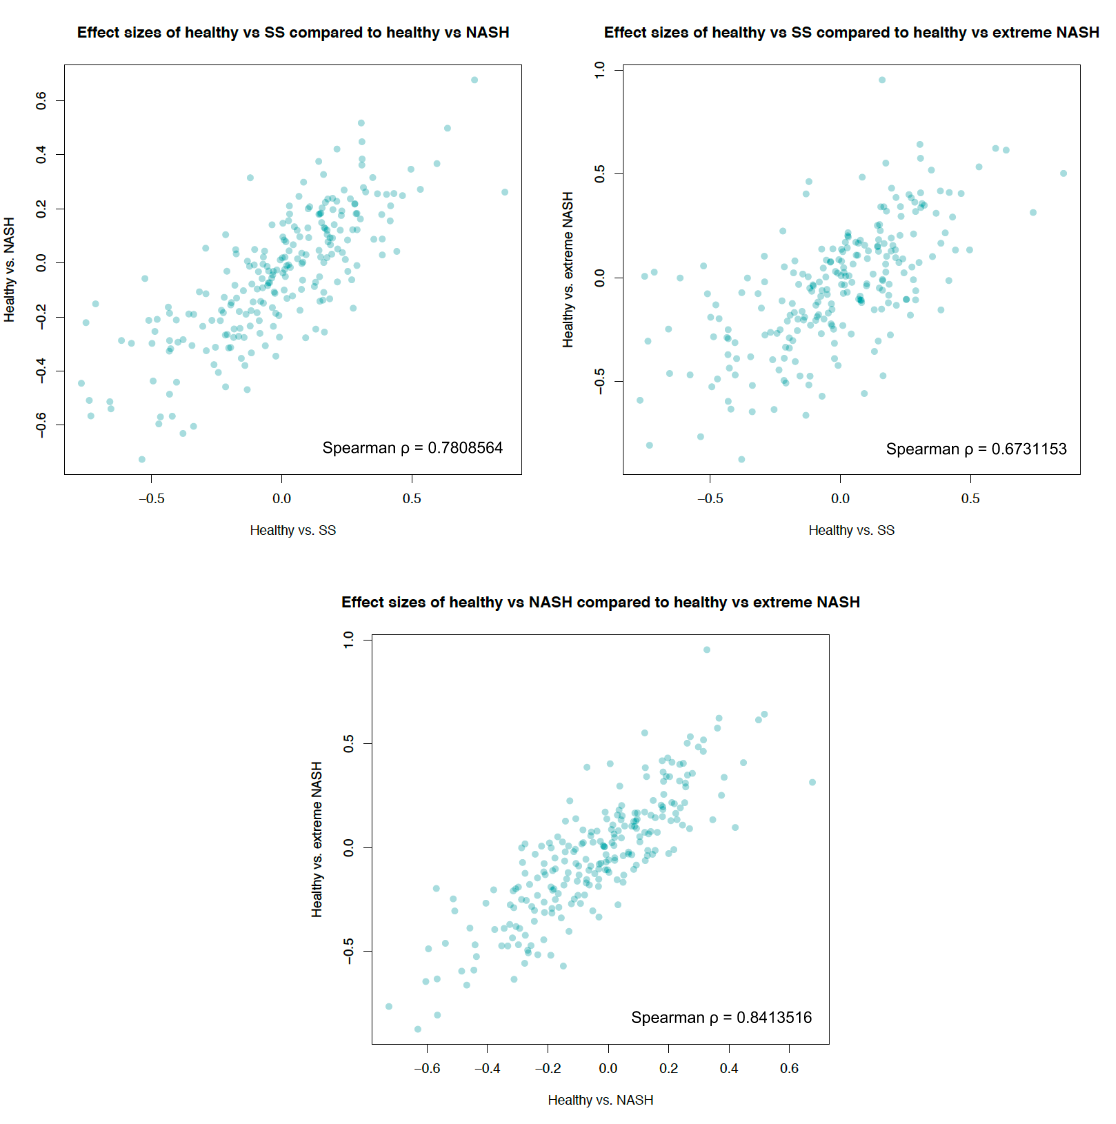
\includegraphics[width=0.95\textwidth]{nafld_16s_effect_sizes.png}
\caption{\textbf{Correlation in effect sizes of different group experiments.} Each point represents one OTU, and the effect size of that OTU in one comparison (for example, comparing the gut microbiome of healthy patients with patients who have simple steatosis) is plotted against the effect size of that OTU in another comparison. The healthy samples used for these comparisons are the 10 healthy samples used for the metagenomic study. The extreme NASH samples used for these comparisons are the subset of the NASH patients selected for the metegenomic study. The y intercepts of the regression lines are all between 0.005 and 0.025, close to zero. The median difference in the absolute effect sizes is -0.02076 for Healthy vs. NASH - Healthy vs. SS, 0.017070 for Healthy vs. extreme NASH - Healthy vs. SS, and 0.04256 for Healthy vs. extreme NASH - Healthy vs. NASH.}
\end{center}
\label{nafld_fig4}
\end{figure}

A differential expression analysis performed with ALDEx2 yielded no significantly differentially abundant OTUs (Fig.~\ref{nafld_fig3}). However, the effect size of each OTU in each comparison is correlated, and the regression line indicates that the effect sizes are higher in the Healthy vs. extreme NASH compared to the Healthy vs. SS or Healthy vs. NASH comparison.

\subsection{Metagenomic experiment}

\paragraph{MetaPhlAn}\mbox{}\\

We ran the metagenomic sequences through MetaPhlAn to infer what the results would be with 16S rRNA gene tag sequencing, so that we could compare with our empirical 16S rRNA gene tag sequencing results. The effect size Spearman coefficient (Fig.~\ref{nafld_metaphlan_effect}) is smaller than the effect size coefficient between the healthy vs. SS and healthy vs. NASH comparison, even though in this case the same samples are being compared.

\begin{figure}[h]
\begin{center}
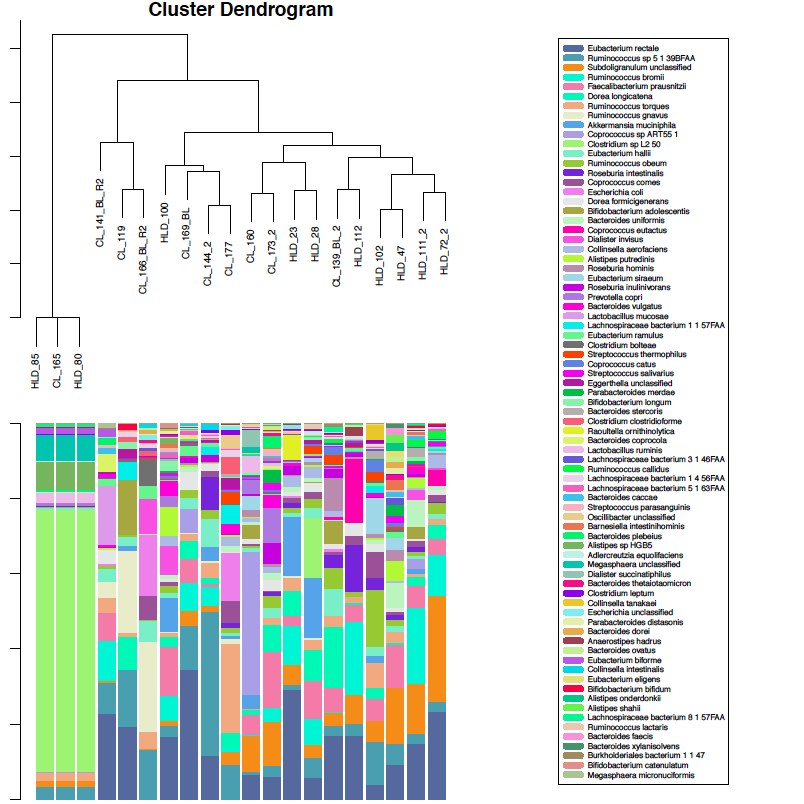
\includegraphics[width=0.95\textwidth]{metaphlan_barplot_dendogram.png}
\caption{\textbf{Taxa barplot dendogram derived from MetaPhlAn.} The metagenomic reads were input into MetaPhlAn to generate a count table. The taxa in the count table were filtered such that only taxa with at least 1\% abundance in any sample was kept. Note that three samples were output to have exactly the same counts (HLD\_80, HLD\_85, and CL\_165), despite not all being in the same condition.}
\end{center}
\label{nafld_metaphlan_barplot}
\end{figure}

\begin{figure}[h]
\begin{center}
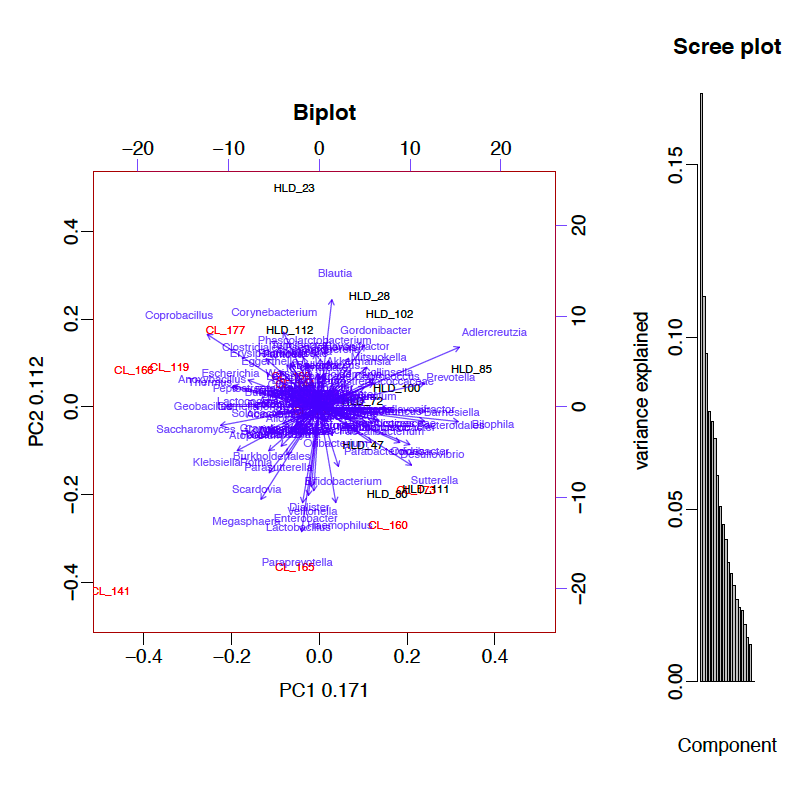
\includegraphics[width=0.95\textwidth]{metaphlan_biplot.png}
\caption{\textbf{Biplot derived from MetaPhlAn.} This biplot was generated from the count table inferred by MetaPhlAn, with taxa filtered such that only taxa with at least 1\% abundance in any sample was kept. Note that the variance explaiend by the first and the second coordinate is not particularly high, indicating that there is not a clear unidirectional separation between groups. Samples from healthy controls are colored black while samples from patients with NASH are colored red.}
\end{center}
\label{nafld_metaphlan_biplot}
\end{figure}

\begin{figure}[h]
\begin{center}
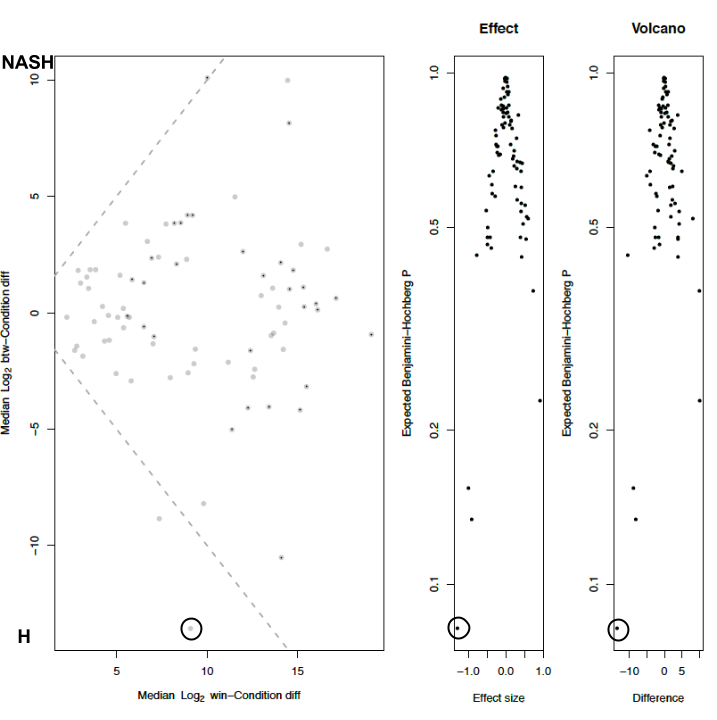
\includegraphics[width=0.95\textwidth]{metaphlan_aldex.png}
\caption{\textbf{Difference within groups vs. difference between groups per taxa, derived from MetaPhlAn.} This plot was generated from the count table inferred by MetaPhlAn, with taxa filtered such that only taxa with at least 1\% abundance in any sample was kept. No taxa are more differential between groups than within groups.}
\end{center}
\label{nafld_metaphlan_aldex}
\end{figure}

\begin{figure}[h]
\begin{center}
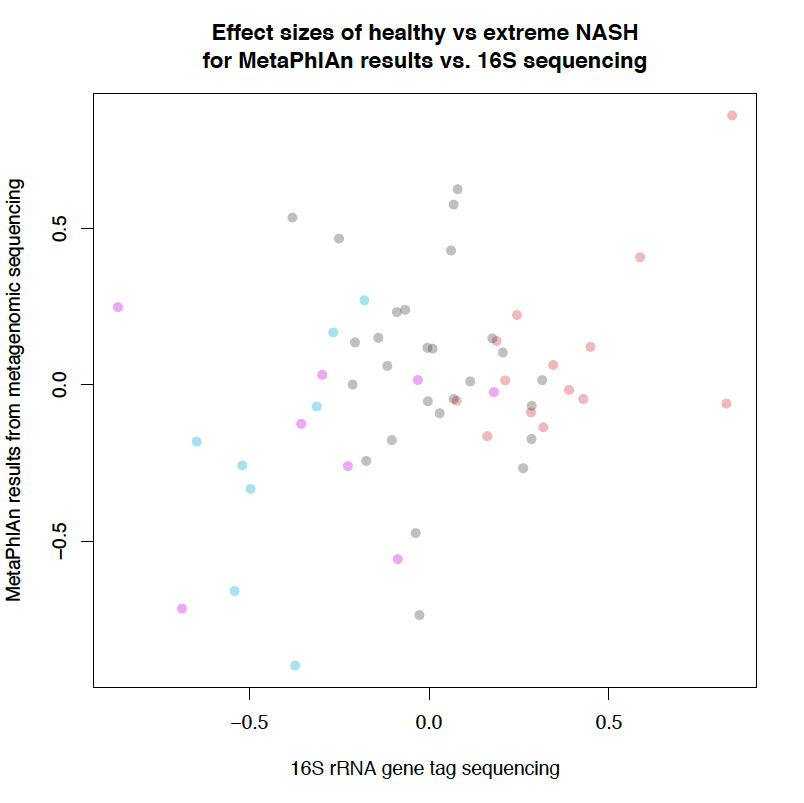
\includegraphics[width=0.95\textwidth]{metaphlan_16s_effects.png}
\caption{\textbf{Effect size correlation between MetaPhlAn and 16S rRNA gene tag sequencing.} For this plot, taxa were amalgamated at the genus level. The Spearman coefficient is 0.5193331. The three samples with identical counts have been removed (otherwise the Spearman coefficent would have been 0.4456304).}
\end{center}
\label{nafld_metaphlan_effect}
\end{figure}

\section{Discussion}

Given the inconsistency in the five papers that have been published about NAFLD and the gut microbiome, we have performed our analysis with care in an effort to find true effects. We found that there was no significant difference between groups by sample clustering (Fig.~\ref{nafld_fig2}) or at the level of the individual OTUs (Fig.~\ref{nafld_fig3}).

There are several factors that would make such a study underpowered. First, the gut microbiome is highly diverse between individuals. This is compounded by the fact that the samples were taken from a diverse Toronto population, including people who immigrated from other countries who likely have different diets. Additionally, the nature of microbiome data is that there are very many more variables (in the form of OTUs or annotated gene functions) than samples.

From Fig.~\ref{nafld_fig4}, the correlation shows that even though there is not enough power to detect a significant difference, the difference from the healthy baseline are moving in the same direction through simple steatosis to nonalcoholic steatohepatitis to extreme NASH.

We hypothesize that there is a characterizable difference in the gut microbiome between patients prone to NASH and healthy controls. Further study with a higher sample size, a more homogenous population, and a greater phenotypic difference between groups may provide the statistical power required to detect the nature of this difference.
